%%%%%%%%%%%%%%%%%%%%%%%%%%%%%%%%%%%%%%%%%
%
% Funkcionalna verifikacija hardvera
% 
%%%%%%%%%%%%%%%%%%%%%%%%%%%%%%%%%%%%%%%%%

Ova vežba je posvećena opisu komunikacije između drajvera i sekvencera, opisu
sekvenci i opisu raznih mogućnosti UVM-a u pogledu pisanja i korišćenja
sekvenci. Dat je i opis mehanizma završetka testa.

%========================================================================================
% Section
%========================================================================================

\section{Drajver - sekvencer interakcija}

U ovom poglavlju je dat kratak pregled drajvera i sekvencera, ukratko je opisana
njihova konekcija i opisane su često korišćene UVM konstrukcije. Sledeća vežba
je posvećena UVM drajveru, a u ovoj vežbi je dat samo kratak pregled kako bi se
razumela struktura sekvenci.

% ----------------------------------------------------------------------------------------

\subsection{Drajver}

Drajver je aktivna komponenta koja emulira signale koji se šalju dizajnu. Na
osnovu podataka iz \emph{sequence item}-a i semplovanja signal na interfejsu,
postavlja signale na ulaze dizajna koji se verifikuje. Transakcije koje prima su
obično na višem nivou apstrakcije, pa se vrši konverzija na pin-nivo apstrakcije
kako bi se ispravno generisali signali. Drajver je preko TLM porta povezan na
sekvencer kako bi vršio komunikaciju i sadrži virtuelni interfejs kako bi
generisao signale. U UVM-u se drajver implementira nasleđujući
\emph{uvm\(\_\)driver \(\#\)(REQ,RSP)} klasu, koja je parametrizovana tipom
transakcija koju će drajver zahtevati i odgovarati (engl. \emph{request},
\emph{response}). Ukoliko se navede samo REQ i RSP će biti istog tipa kao i REQ.
Npr:

\begin{lstlisting}
class calc_driver extends uvm_driver#(calc_seq_item);
  // ...
endclass : calc_driver
\end{lstlisting}

Napomena: u SystemVerilog-u se parametrizacija vrši koristeći ``\(\#\)'' znak.
Nalik C++-su ovim mehanizmom se omogućava pisanje generičkih klasi kojima će se
stvarna vrednost parametra proslediti tek prilikom korišćenja. Primer
deklarisanja parametrizovane klase:

\begin{lstlisting}
class param_example #(type T = int, type G = bit, int A = 10);
\end{lstlisting}

% ----------------------------------------------------------------------------------------

\subsection{Sekvencer}

Sekvencer koristi sekvence kako bi poslao podatke drajveru, ali i prima odgovor
od drajvera ukoliko je to potrebno čime se omogućava kreiranje korisnih
stimulusa. Sekvencer služi kao ariber čiji je zadatak kontrola slanja
transakcija iz jedne ili više sekvenci.\\

U praksi najčešće nije potrebno modifikovati sekvencer jer su funkcionalnosti
koje se nalaze u \emph{uvm\(\_\)sequencer} klasi obično dovoljne. Kao i drajver,
i sekvencer je moguće parametrizovati sa tipom transakcije, npr:

\begin{lstlisting}
class calc_sequencer extends uvm_sequencer#(calc_seq_item);
  // ...
endclass : calc_sequencer
\end{lstlisting}

Ukoliko, osim parametrizacije, nije potrebno ubacivati dodatni sadržaj u
sekvencer, često se samo koristi \emph{typedef} naredba kako bi se izbegao
nepotrebni kod, npr:

\begin{lstlisting}
typedef uvm_sequencer#(calc_seq_item) calc_sequencer;
\end{lstlisting}

% ----------------------------------------------------------------------------------------

\subsection{Komunikacija}

UVM komponente komuniciraju preko standardnih TLM (engl. \emph{transaction level
  modeling}) interfejsa koji olakšava povezivanje i ponovno korišćenje.
Komponenta može komunicirati preko svog interfejsa sa bilo kojom drugom
komponentom koja implementira taj interfejs. U praksi je ovaj način komunikacije
veoma čest za drajver - sekvencer interakciju i monitor - \emph{scoreboard}
komunikaciju. U ovoj i narednoj vežbi je fokus na komunikaciji između drajvera
i sekvencera, dok je detaljan opis rada TLM konekcija ostavljen za vežbu o
monitoru.\\

U \emph{uvm\(\_\)driver} i \emph{uvm\(\_\)sequencer} klasama postoji deklaracija
odgovarajućih portova i ugrađena logika oko komunikacije, tako da je upotreba
od strane korisnika veoma jednostavna. Potrebno je samo povezati drajver i
sekvencer, koristeći metodu \emph{connect}. Povezivanje se tipično vrši u
\emph{connect} fazi, gde je, na primeru ispod, \emph{driver} instanca prethodno
kreiranog drajvera, a \emph{sequencer} instanca prethodno kreiranog sekvencera.
\emph{seq\(\_\)item\(\_\)port} i \emph{seq\(\_\)item\(\_\)export} su imena
nasleđenih TLM portova.

\begin{lstlisting}
function void connect_phase(uvm_phase phase);
  drviver.seq_item_port.connect(sequencer.seq_item_export);
endfunction : connect_phase
\end{lstlisting}

Sam UVM ne pruža samo mogućnost korišćenja bibilioteke, već i definiše način
upotrebe kako bi se kreirale univerzalne verifikacione komponente koje će
pratiti datu metodologiju. S tim u vezi, postoji jasno definisana komunikacija
između drajvera i sekvencera, koristeći određene UVM funkcije, čiji je opis
dat u nastavku.\\

UVM drajver sadrži mnoge metode za komunikaciju sa sekvencerom. Najčešće
korišćene su:

\begin{itemize}
\item \emph{get\(\_\)next\(\_\)item()} - blokirajuća metoda koja traži novi
  objekat; vraća pokazivač na novi REQ objekat
\item \emph{try\(\_\)next\(\_\)item()} - neblokirajuća verzija koja vraća
  \emph{null} pokazivač ukoliko nema dostupnog objekta
\item \emph{item\(\_\)done()} - neblokirajuća metoda koja završava proces
  rukovanja između drajvera i sekvencera; poziva se nakon
  \emph{get\(\_\)next\(\_\)item()} ili uspešnog \emph{try\(\_\)next\(\_\)item()}
\end{itemize}

Sam sekvencer služi za arbitraciju, dok se \emph{sequence item} objekti kreiraju
i kontrolišu iz sekvenci.  Da bi se paket poslao drajveru, on mora proći kroz
nekoliko koraka:

\begin{enumerate}
\item Kreiranje - veoma je bitno kreirati paket koristeći \emph{factory} kako bi
  se olakšala ponovna upotreba odnosno kako bi se dozvolio \emph{override} metod
  ukoliko je to potrebno (objašnjeno u narednim vežbama)
\item \emph{Start\(\_\)item()} - blokirajući poziv koji čeka da se uspostavi
  veza sa drajverom. Sekvenceru šalje pokazivač na sledeći objekat
\item Randomizacija paketa ukoliko je to potrebno
\item \emph{Finish\(\_\)item()} - blokirajući poziv koji čeka da drajver završi
  sa paketom (napomena: \emph{start\(\_\)item()} i \emph{finish\(\_\)item()}
  čekaju na drajver kako bi se osigurao korektan transfer paketa, ali oni ne
  troše simulaciono vreme)
\item \emph{Get\(\_\)response()} - opcioni poziv ako je potrebno da drajver
  pošalje odgovor sekvenceru
\end{enumerate}

\begin{figure}[h!]
  \centering
  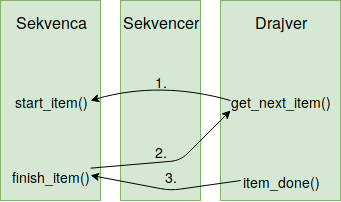
\includegraphics[width=60mm, scale=0.5]{img/v6_drv_seq_flow.png}
  \caption{Drajver-sekvencer \emph{flow}}
  \label{fig:drv_seq_flow}
\end{figure}

Preporučeni \emph{flow} je prikazan na slici \ref{fig:drv_seq_flow}. Drajver
traži transakciju od sekvencera koristeći \emph{get\(\_\)next\(\_\)item()},
obrađuje istu i zatim kompletira \emph{handshake} koristeći
\emph{item\(\_\)done()} čime signalizira sekvenceru da je objekat obrađen. Sa
druge strane, u sekvenci se kreiraju transakcije prateći prethodne korake. Kada
drajver pozove \emph{item\(\_\)done()}, odblokiraće se \emph{finish\(\_\)item()}
metoda u sekvenci i može se nastaviti sa izvršavanjem.\\

Pored ovog načina, moguće je ostvariti komunikaciju koristeći \emph{peek()},
\emph{put()} i \emph{get()} metode u drajveru koje su opisane u narednoj vežbi.\\

%========================================================================================
% Section
%========================================================================================

\section{Sekvence}

Sekvence su objekti (ne komponente) koje sadrže logiku generisanja stimulusa.
Kao i većina UVM okruženja, i kod sekvenci postoji preporučen način upotrebe,
kako u pogledu strukture same sekvence, tako i za sam način generisanja
stimulusa. U ovom poglavlju je opisan mehanizam generisanja stimulusa, dat je
pregled strukture sekvenci i objašnjene često korišćene funkcije.

% ----------------------------------------------------------------------------------------

\subsection{Struktura}

Sve sekvence u okruženju treba da, direktno ili indirektno, nasleđuju
\emph{uvm\(\_\)sequence} klasu. Pošto sekvence nisu komponente one ne sadrže UVM
faze, međutim ipak postoji sličan mehanizam koji garantuje ispravan rad i
ispravnu komunikaciju sa drajverom. Tri najčešće korišćene metode su
\emph{pre\(\_\)body()}, \emph{body()} i \emph{post\(\_\)body()}. Glavna logika
treba da se nalazi u \emph{body()} tasku. \emph{Pre\(\_\)body()} i
\emph{post\(\_\)body()} su taskovi koji se pozivaju pre, odnosno posle
\emph{body()} taska. Kao i kod pisanja testova, dobra je praksa da postoji bazna
klasa u kojoj se deklariše sekvencer, vrši eventualno podizanje/spuštanje
prigovora (\emph{raise / drop objection}, opisano u narednom poglavlju), kao i
sve ostale radnje koje će se ponavljati u svim sekvencama.

\begin{lstlisting}
class calc_seq extends uvm_sequence#(calc_seq_item);

  `uvm_object_utils(calc_seq)
  `uvm_declare_p_sequencer(calc_sequencer)

  function new(string name = "calc_seq");
    super.new(name);
  endfunction

  virtual task pre_body();
    // ...
  endtask : pre_body

  // transaction generating logic in body
  virtual task body();
    // calls to uvm_do or uvm_do with macro
    // or start / finish item
    // ...
  endtask : body

  virtual task post_body();
    // ...
  endtask : post_body

endclass : calc_seq
\end{lstlisting}

Kao i kod drajvera i sekvencera, potrebno je parametrizovati sekvence tipom
\emph{sequence\(\_\)item}-a koji će se generisati. Ovo, između ostalog,
omogućava korišćenje podrazumevanog objekta u sekvencama. Pored \emph{factory}
registracije (\emph{\`\ uvm\(\_\)object\(\_\)utils(calc\(\_\)seq)} u primeru),
potrebno je i deklarisati sekvencer koji će se koristiti. Svaka sekvenca se pri
pokretanju veže za odgovarajući sekvencer kome se može pristupati preko
pokazivača. Ovaj korak je moguće i izostaviti, ili deklarisati sekvencere na
drugi način, međutim najjednostavniji način za naše potrebe je da se deklariše
takozvani \emph{p sekvencer} koristeći odgovarajući makro
(\emph{\`\ uvm\(\_\)declare\(\_\)p\(\_\)sequencer(calc\(\_\)sequencer)}, gde
\emph{calc\(\_\)sequencer} predstavlja ime korišćenog sekvencera).

% ----------------------------------------------------------------------------------------

\subsection{Generisanje stimulusa}

U prethodnom poglavlju smo videli da je za generisanje transakcije potrebno
ispratiti nekoliko koraka:

\begin{enumerate}
\item Kreiranje - veoma je bitno kreirati paket koristeći \emph{factory} kako bi
  se olakšala ponovna upotreba odnosno kako bi se dozvolio \emph{override} metod
  ukoliko je to potrebno (objašnjeno u narednim vežbama)
\item \emph{Start\(\_\)item()} - blokirajući poziv koji čeka da se uspostavi
  veza sa drajverom. Sekvenceru šalje pokazivač na sledeći objekat
\item Randomizacija paketa ukoliko je to potrebno
\item \emph{Finish\(\_\)item()} - blokirajući poziv koji čeka da drajver završi
  sa paketom (napomena: \emph{start\(\_\)item()} i \emph{finish\(\_\)item()}
  čekaju na drajver kako bi se osigurao korektan transfer paketa, ali oni ne
  troše simulaciono vreme)
\item \emph{Get\(\_\)response()} - opcioni poziv ako je potrebno da drajver
  pošalje odgovor sekvenceru
\end{enumerate}

Prva četiri koraka su obavezna, dok je peti opcioni i koristi se samo ukoliko za
dato okruženje postoji potreba prikupljanja odgovora od drajvera. Logika
generisanja stimulusa treba da se nalazi u \emph{body()} tasku, npr:

\begin{lstlisting}
virtual task body();

  calc_seq_item calc_it;

  // prvi korak kreiranje transakcije
  calc_it = calc_seq_item::type_id::create("calc_it");

  // drugi korak - start
  start_item(calc_it);

  // treci korak priprema
  // po potrebi moguce prosiriti sa npr. inline ogranicenjima
  assert(calc_it.randomize());

  // cetvrti korak - finish
  finish_item(calc_it);

endtask: body
\end{lstlisting}

Pošto se ova četiri koraka često ponavljaju tj. standardni su za interakciju
drajvera i sekvencera, razvijeni su odgovarajući UVM makroi kao bi se izbeglo
nepotrebno ponavljanje koda i povećala čitljivost. Iako veoma korisni, makroi
ipak uvode neka ograničenja pri korišćenju, tako da je nekad ipak potrebno ručno
odraditi ove korake. ``UVM Cookbook'' ne preporučuje upotrebu makroa, ali su oni
česti u praksi.

\subsubsection{\emph{\`\ uvm\(\_\)do}}

\emph{\`\ uvm\(\_\)do} makro kao argument prima \emph{sequence\(\_\)item}. Kada se
nasledi i parametrizuje \emph{uvm\(\_\)sequence} klasa, nasleđuje se i instanca
objekta pod nazivom \emph{req} čiji je tip upravo parametar koji smo prosledili.
Što znači da u svakoj sekvenci već postoji objekat \emph{req} koji se može
koristiti za komunikaciju. Slično postoji i objekat \emph{rsp} koji treba
koristiti za odgovor ukoliko je isti potreban. Upotreba \emph{\`\ uvm\(\_\)do}
makroa je:

\begin{lstlisting}
virtual task body();
  `uvm_do(req)
endtask : body
\end{lstlisting}

Ovim se postiže generisanje i slanje jedne transakcije drajveru, koja će se
zatim generisati na interfejsu.

\subsubsection{\emph{\`\ uvm\(\_\)do\(\_\)with}}

Ukoliko je potrebna veća kontrola prilikom slanja transakcije, moguće je
koristiti \emph{\`\ uvm\(\_\)do\(\_\)with} makro, koji osim
\emph{sequence\(\_\)item} argumenta prima i bilo koje validno inline
ograničenje. Npr:

\begin{lstlisting}
virtual task body();
  `uvm_do_with(req, { req.data == 16'h5A5A; } )
endtask : body
\end{lstlisting}

U ovom primeru se šalje jedna transakcija pri čemu je vrednost \emph{data} polja
ograničena na 16\textquotesingle h5A5A.

\subsubsection{Kontrola}

U prethodnim primerima smo slali samo jednu transakciju. Često je neophodno
omogućiti veću kontrolu nad izvršavanjem sekvenci - omogućiti kontrolisanu
randomizaciju, slanje željenog broja transakcija itd. Prilikom pisanja sekvenci
moguće je koristiti sve mogućnosti koje SystemVerilog pruža. U nastavku je dato
par konstrukcija koje se često sreću i koje daju uvid u ove mogućnosti.\\

Kontrola prilikom randomizacije je često vrši pomoću \emph{rand} polja u
sekvenci, kako bi se omogućila laka kontrola direktno iz testa koji startuje
sekvencu. Sledeći primer ilustruje slanje više transakcija.

\begin{lstlisting}
class calc_simple_seq extends calc_base_seq;

  `uvm_object_utils (calc_simple_seq)

  rand int unsigned num_of_tr;

  constraint num_of_tr_con { num_of_tr inside { [1:100] }; }

  function new(string name = "calc_simple_seq");
    super.new(name);
  endfunction

  virtual task body();
    repeat(num_of_tr) begin
      `uvm_do(req);
    end
  endtask : body

endclass : calc_simple_seq
\end{lstlisting}

Takođe je moguće pozivati jednu sekvencu iz druge, pri čemu je moguće koristiti
prethodno opisane makroe i nad sekvencama (ili koristiti metodu \emph{start}
opisanu u narednom poglavlju).

\begin{lstlisting}
class calc_simple_seq extends calc_base_seq;

  `uvm_object_utils (calc_simple_seq)

  calc_sub_seq sub_seq;

  function new(string name = "calc_simple_seq");
    super.new(name);
  endfunction

  virtual task body();
    `uvm_do(sub_seq);
  endtask : body

endclass : calc_simple_seq
\end{lstlisting}

% ----------------------------------------------------------------------------------------

\subsection{Pokretanje sekvenci}

Sekvence se pokreću ili iz testa ili iz drugih sekvenci. Postoje dva glavna
načina pokretanja sekvenci - eksplicitno koristeći \emph{start} metodu ili
implicitno kao podrazumevanu sekvencu.\\

Ukoliko je potrebna veća kontrola pokretanja sekvenci (npr. podešavanje
parametara, trenutak startovanja, ...) preporučuje se eksplicitno pokretanje
sekvence korišćenjem \emph{start} metode, npr:

\lstinputlisting[caption=\emph{Start}\(\_\)metoda, label=lst:v6_test_simple]{code/tests/v6_test_simple.sv}

Prilikom poziva \emph{start} metode jedini obavezan argument je sekvencer na
kome će pokrenuti sekvenca.\\

Što se tiče podrazumevanih sekvenci, one se uglavnom navode u \emph{build} fazi
testa, npr:

\lstinputlisting[caption=Podrazumevane\(\_\)sekvence, label=lst:v6_test_simple_2]{code/tests/v6_test_simple_2.sv}

Za navođenje podrazumevane sekvence se koriti UVM \emph{configuration database}
koji omogućava postavljanje konfiguracionih parametara u okruženju, u našem
slučaju podrazumevane sekvence (\emph{uvm\(\_\)config\(\_\)db} će biti
detaljnije obrađen u narednim vežbama). U prethodnom primeru je za \emph{main}
fazu prethodno instanciranog \emph{seqr} sekvencera podešena
\emph{calc\(\_\)simple\(\_\)seq} kao podrazumevana sekvenca.\\

Pokretanje podrazumevanih sekvenci je u UVM-u nasleđeno iz OVM-a i zadržano je
radi lakšeg prelaza sa jedne metodologije na drugu.
Iako i dalje često korišćeno, preporuka je koristiti \emph{start} metodu radi bolje kontrole.

%========================================================================================
% Section
%========================================================================================

\section{Mehanizam završetka testa}

Svaki testbenč koji koristi standardne UVM faze se sastoji od nekoliko faza za
kreiranje i povezivanje koje se izvršavaju u nultom vremenu, zatim određen broj
faza koje troše vreme, kao i nekoliko faza za završetak testa koje se izvršavaju
u nultom vremenu. Do kraja testa će doći kada se završe sve faze koje troše
vreme, a svaka faza se završava kada nema prigovora za tu fazu što znači da se
kraj testa kontroliše podizanjem i spuštanjem prigovora. Komponenta ili sekvenca
će podići prigovor na početku aktivnosti koja se mora završiti u datoj fazi, a
spustiti prigovor po završetku te aktivnosti. Tek kada se svi podignuti
prigovori spuste, moguće je završiti datu fazu. U praksi se često dešava da je
faza samo trenutno bez prigovora tj. da će se uskoro podići još neki prigovor i
da ne treba odmah završiti sa trenutnom fazom. U tom slučaju se može postaviti
vreme čekanja (engl. \emph{drain time}) koje unosi kašnjenje za završetak faze.
Ako u tom vremenskom intervalu podigne prigovor, faza se neće završiti i opet će
se čekati na spuštanje svih prigovora.\\

Kontrola prigovora se uglavnom vrši ili iz samog testa ili iz sekvenci.
Kontrola iz testa se često sreće kada se sekvence eksplicitno pokreću.
Jedan primer je prikazan ispod.

\begin{lstlisting}
task main_phase(uvm_phase phase);
  phase.raise_objection(); //rasing objection
  example_seq.start(example_agent.sequencer);
  phase.drop_objection(); //droping objection
endtask
\end{lstlisting}

Što se tiče kontrole iz sekvenci sekvenci, pošto se čitava logika generisanja
stimulusa nalazi u \emph{body()} tasku, prigovor je potrebno podići pre odnosno
posle izvršavanja \emph{body()} taska i ovo se najčešće radi u
\emph{pre\(\_\)body()} odnosno \emph{post\(\_\)body()} taskovima.
Ovaj kod se najčešće nalazi u baznoj sekvenci kako bi se prigovori generisali
prilikom pokretanja svake sekvence.
Test se tada neće završiti do god postoje sekvence u okruženju koje nisu
završile sa generisanjem stimulusa.

\begin{lstlisting}
// objections are raised in pre_body
virtual task pre_body();
  uvm_phase phase = get_starting_phase();
  if (phase != null)
    phase.raise_objection(this, {"Running sequence '", get_full_name(), "'"});
    uvm_test_done.set_drain_time(this, 200ns)
endtask : pre_body

// objections are dropped in post_body
virtual task post_body();
  uvm_phase phase = get_starting_phase();
  if (phase != null)
    phase.drop_objection(this, {"Completed sequence '", get_full_name(), "'"});
endtask : post_body
\end{lstlisting}

Jedan način podizanja / spuštanja prigovora je prikazan kodom iznad. Koriste se
\emph{raise\(\_\)objection/drop\(\_\)objection} metode.
\emph{starting\(\_\)phase} je član bazne klase koji će biti ispravno postavljen
jedino ukoliko je sekvenca pokrenuta kao podrazumevana (\emph{default}) za neku
fazu.\\

Pomoću metode \emph{set\(\_\)drain\(\_\)time} se postavlja takozvano
\emph{drain} vreme koje u datom primeru unosi toleranciju od 200 ns, odnosno
nakon spuštanja poslednjeg prigovora test se neće odmah završiti nego će se
sačekati još 200 ns zbog mogućnosti da se u tom periodu ponovo podigne neki
prigovor.\\

Napomena: pošto je sekvenca ručno pokrenuta, \emph{starting\(\_\)phase} polje iz
prethodnog kodnog fragmenta bi imalo vrednost \emph{null} tako da se korišćenjem
oba kodna fragmenta ispovremeno ne bi podigla dva prigovora za istu sekvencu.\\

Napomena: podizanje / spuštanje prigovora u sekvenci se često koristi uz UVM 1.1
biblioteku. Za UVM 1.2 preporučen način je podizanje / spuštanje prigovora iz
testa.

%========================================================================================
% Section
%========================================================================================

\section{Zadaci}

\paragraph{Zadatak}

Napisati sekvence koje će se koristiti za verifikaciju ``Calc1'' DUT-a,
uključujući:

\begin{itemize}
\item Sekvenca za generisanje jedne transakcije na nasumično izabranom portu, sa
  nasumičnim podacima i komandom
\item Sekvenca za  generisanje više nasumičnih transakcija na istom portu
\item Sekvenca za generisanje više nasumičnih transakcija, pri čemu se broj
  transakcija nalazi u opsegu (1, 10), a svaka naredna transakcija se nalazi na
  portu različitom od prethodnog
\item Sekvenca za  generisanje više nasumičnih transakcija pri čemu su komande
  uvek za jednu ALU, bez kašnjenja između generisanja transakcija
\item smisliti još nekoliko primera sekvenci koji bi mogle biti korisne za
  verifikaciju
\end{itemize}

\paragraph{Zadatak}

Napisati test (uz eventualne pomoćne testove ili sekvence) u kome će se poslati
tačno 8 transakcija, koristeći neku od prethodno razvijenih sekvenci. Na koje je
načine ovo moguće odraditi?

%========================================================================================
% Section
%========================================================================================

\section{Appendix}

\lstinputlisting[caption=calc\(\_\)if, label=lst:calc_if]{code/calc_if.sv}
\lstinputlisting[caption=v6\(\_\)calc\(\_\)sequencer, label=lst:v6_sequencer]{code/v6_calc_sequencer.sv}
\lstinputlisting[caption=v6\(\_\)calc\(\_\)driver, label=lst:v6_driver]{code/v6_calc_driver.sv}
\lstinputlisting[caption=v6\(\_\)calc\(\_\)seq\(\_\)item, label=lst:v6_seq_item]{code/v6_calc_seq_item.sv}
\lstinputlisting[caption=v6\(\_\)test\(\_\)base, label=lst:v6_test_base]{code/tests/v6_test_base.sv}
\lstinputlisting[caption=v6\(\_\)test\(\_\)simple, label=lst:v6_test_simple]{code/tests/v6_test_simple.sv}
\lstinputlisting[caption=v6\(\_\)test\(\_\)simple\(\_\)2, label=lst:v6_test_simple_2]{code/tests/v6_test_simple_2.sv}
\lstinputlisting[caption=v6\(\_\)test\(\_\)lib, label=lst:v6_test_lib]{code/tests/v6_test_lib.sv}
\lstinputlisting[caption=v6\(\_\)calc\(\_\)base\(\_\)seq, label=lst:v6_calc_base_seq]{code/sequences/v6_calc_base_seq.sv}
\lstinputlisting[caption=v6\(\_\)calc\(\_\)simple\(\_\)seq, label=lst:v6_calc_simple_seq]{code/sequences/v6_calc_simple_seq.sv}
\lstinputlisting[caption=v6\(\_\)calc\(\_\)seq\(\_\)lib, label=lst:v6_calc_seq_lib]{code/sequences/v6_calc_seq_lib.sv}
\lstinputlisting[caption=v6\(\_\)calc\(\_\)verif\(\_\)pkg, label=lst:v6_calc_verif_pkg]{code/v6_calc_verif_pkg.sv}
\lstinputlisting[caption=v6\(\_\)calc\(\_\)verif\(\_\)top, label=lst:v6_calc_verif_top]{code/v6_calc_verif_top.sv}
\lstinputlisting[language=tcl, caption=calc\(\_\)run, label=lst:calc_run]{code/calc_run.do}

%========================================================================================

